\documentclass[10pt]{article}
% \def\StudentVersion{}
\usepackage{../common}
\makeatletter

\def\LecStr{Alexander Rush}
\def\LecNum{1}
\def\LecTitle{Lectures Notes on Search}
\def\LecDate{}

\def\Graph{\path node(A)[draw, initial, state] at (-2, 1) {A};
    \path node(B)[draw, state] at (-1, 3) {B};
    \path node(C)[draw, state, accepting] at (4, 2) {C};
    \path node(D)[draw, state] at (1, 1) {D};
    \path node(E)[draw, state] at (2, 3) {E};
    \path[draw] (A) --node[xshift=-0.2cm]{2} (B); 
    \path[draw] (B) --node[yshift=0.2cm]{4} (E); 
    \path[draw] (A) --node[yshift=0.2cm]{3} (D); 
    \path[draw] (A) --node[yshift=0.2cm]{5} (E); 
    \path[draw] (D) --node[yshift=0.2cm]{4} (C); 
    \path[draw] (E) --node[yshift=0.2cm]{4} (C); 
}

\def\Words{
  \matrix(dict)[matrix of nodes, ampersand replacement=\&]{
    Mary \& golpeo \& la \& bruja \& verde \\
    ~\\
    ~\\
    Mary \& slapped \& the \& green \& witch \\ };
}

\begin{document}
\MakeScribeTop{}

\section{Summary Board}

\begin{itemize}
\item Search Model
\item Paths and Costs
\item Example 1
\item Example 2
\item Review: Containers
\item Search Algorithms
\end{itemize}

\section{Introduction}

The structure of the lectures:

\begin{itemize}
\item Models
\item Algorithms
\end{itemize}

Future Topics of search: 

\begin{itemize}
\item Pure Search, Game-Playing, Constraint Satisfaction, Logical Inference
\end{itemize}

Note on Notation

\begin{itemize}
\item Please stop me this class for notational questions...
\end{itemize}

\section{Board 1}

\begin{itemize}
\item MapQuest, google/apple maps
\item Commercial routing
\end{itemize}

\begin{figure}[h]
  \centering
  \begin{tikzpicture}
    \Graph
  \end{tikzpicture}
  \label{fig:minigraph}
\end{figure}



\section{Board 2}
 \air
\textbf{Search Model}
\begin{center}
\begin{tabularx}{\linewidth}{llX}
  \toprule
  Name (AIMA) & Type & Description \\
  \midrule
\\
 State space & $\mcS$ & Set of states of world. \\\\
 Action space & $\mcA$& Set of actions in world. \\\\
 Action model&  $\msc{Act}: \mcS \mapsto 2^\mcA$ & Actions applicable at a state \\\\
 Transition model&  $\msc{Res}:  \mcS \times \mcA \mapsto \mcS $ &   Result of taking action at state (stop an explain).  \\\\
 Initial state &  $s_0 \in \mcS$ & Starting State of world.  \\\\
 Goal test& $\msc{Goal}: \mcS \rightarrow \{0, 1\}$ & Is state a goal? \\\\
 \bottomrule
\end{tabularx}
\end{center}
(Stop and make clear the function notation)

\air

\begin{itemize}
\item  Start: $s_0$,
\item Take any action $a \in \msc{Act}(s_0)$
\item New state $s_1 \gets \msc{Res}(s_0, a)$
\item Proceed until we reach $\msc{Goal}(s) = 1$
\end{itemize}

\section{Board 3}

\textbf{Paths and Costs}
\begin{defn}
   A \textbf{path}
is a sequence of state-action pairs starting at $s_0$:  \[p = (s_0, a_0), (s_1, a_1), \ldots, (s_{n-1}, a_{n-1}).\] 
\noindent Where $s_i = \msc{Res}(s_{i-1}, a_{i-1})$ for all i and $n$ is the depth. 
Let the set of all paths as $\mcP$.

Let the last state of the path to be  
 \[p_{\mathrm{last}} \triangleq \msc{Act}(s_{n-1}, a_{n-1}).\] 

\end{defn}

\begin{defn}
  A \textbf{solution} is a path that reaches a goal state, that is if $\msc{Goal}(p_{\msc{last}}) = 1$.


  Define the set of solutions as: 
  \[\mcQ = \{p \in \mcP:  \msc{Goal}(p_{\msc{last}}) = 1 \} \]
\end{defn}

(Stop and make clear the set notation)

\section{Board 4}

Costs: example length of the graph

\air

\begin{center}
\begin{tabularx}{\linewidth}{llX}
  \toprule
  \\
 Step cost & $c:\mcS \times \mcA \mapsto \reals_+$ & Cost of action at state. \\\\
 Path cost & $g:\mcP  \mapsto \reals_+$ & Cost of a path, i.e. $g(p) = \sum_{i=0}^{n-1}  c(s_i, a_i)$. \\\\
\bottomrule
\end{tabularx}
\end{center}

Goal: Find the \textbf{optimal solution} or lowest-cost path:

\[ p^* = \argmin_{p \in \mcQ} g(p) \] 

\noindent where $\mcQ$ is the solution set. 


\section{Board 5}

(Pull back down example board)

\textbf{Example 1}
\begin{center}
\begin{tabularx}{\linewidth}{llX}
  \toprule
  Name & Value & Description \\
  \midrule
\\
 State space & \censor{$\mcS = \{\mathrm{A, B, C, D, E}\}$} & \censor{Locations} \\\\
 Action space & \censor{$\mcA = \{ \mathrm{\textsc{Go}(A)}, \mathrm{\textsc{Go}(B)}, \mathrm{\textsc{Go}(C)},\ldots $}& \censor{Move along edge.} \\\\
 Actions&  \censor{$\msc{Act}$} & \censor{Which are possible. For instance, $\msc{Act}(\mathrm{A}) =\{\mathrm{\textsc{Go}(B), \textsc{Go}(D), \textsc{Go}(E)}\}$.} \\\\
 Transition model&  \censor{$\msc{Res} $} &  \censor{Moves to new location. For instance, $\msc{Res}\mathrm{(A, \textsc{Go}(E))} = \mathrm{E}$}    \\\\
 Initial state &  \censor{$s_0 = \mathrm{A}$} & \censor{The initial state A.}  \\\\
 Goal test& \censor{$\msc{Goal}(s)$} & \censor{Gives 1 if state $s$ is C, 0 otherwise.} \\\\
 Step cost & \censor{$c$} & \censor{For instance $c(\mathrm{A, \textsc{Go}(E)}) = 5$, distances.} \\\\
 \bottomrule
\end{tabularx}
\end{center}
\air


\section{Board 6}

A search problem has several associated properties that will help us quantify the difficulty of finding a solution or the optimal solution. 

\air
\begin{center}
\begin{tabularx}{\linewidth}{llX}
  \toprule
  Name & Symbol & Desc \\
  \midrule
\\
 Branching Factor & $b$ & Max actions at a state.  \\\\
 Min Depth &  $d$ & Shallowest solution depth.
 \\\\
 Max Depth & $m$& Deepest solution depth. \\\\
 Optimal Cost & $C^*$& Cost of the optimal solution $g(p^*)$. \\\\
 \bottomrule
\end{tabularx}
\end{center}

\begin{itemize}
\item Min Depth Solution may *not* be optimal
\item We may not know any of these properties exactly.
\end{itemize}

\section{Board 7}
\begin{exercise}
  What are the search properties $b, d, m, C^*$ for the path finding
  problem? Shallowest goal? Deepest goal? Branching factor?
\end{exercise}

\air
\begin{center}
\begin{tabularx}{\linewidth}{llX}
  \toprule
  Name  & Type & Description \\
  \midrule
\\
 Branching Factor & $b$ & \censor{}  \\\\
 Min Depth &  $d$ & \censor{} \\\\
 Max Depth & $m$& \censor{} \\\\
 Optimal Cost & $C^*$& \censor{} \\\\
 \bottomrule
\end{tabularx}
\end{center}


\subsection{Board 8}
\textbf{Example 2}

\begin{itemize}
\item And now for something very different.
\end{itemize}

(Pause, read story about machine translation)


Consider for example, a very different problem: finding the best translation of a Spanish sentence into English. The following figure shows an example of this problem. 

\begin{figure}[h]
  \centering
  \begin{tikzpicture}
    \Words
    \path[draw, ->] (dict-1-1) -> (dict-4-1);
    \path[draw, ->] (dict-1-2) -> (dict-4-2);
    \path[draw, ->] (dict-1-3) -> (dict-4-3);
    \path[draw, ->] (dict-1-4) -> (dict-4-5);
    \path[draw, ->] (dict-1-5) -> (dict-4-4);
  \end{tikzpicture}
  \label{fig:mt}
\end{figure}

Where do the scores come from?
\begin{itemize}
\item Translation Dictionary: Cost of translating each Spanish word. i.e. golpeo => slapped : 1, golpeo => hit : 2, golpeo: slaps: 20

\item Language Model: Cost of two English words being next to each other. i.e. ``the => witch'': 1, "witch => the'': 5, ``the => the'': 100
\end{itemize}


\subsection{Board 9}

Ask people.

\air 
\begin{center}
\begin{tabularx}{\linewidth}{llX}
  \toprule
  Name & Value & Description \\
  \midrule
\\

 State space & $\mcS$ & The English translation AND which words have been translated. \\\\
 Initial state &  $s_0$ & Translation is blank, all words are untranslated.  \\\\
 Action space & $\mcA$& Translate a word . \\\\
 Actions&  $\msc{Act}$ & All ways to translate any unused word. \\\\
 Transition model&  $\msc{Res} $ &  Add word to translation and remove word from source.    \\\\
 Goal test& $\msc{Goal}(s)$ & Any state with all words translated. \\\\
 Step cost & $c$ &  Sum of translation and language model. \\
 \bottomrule
\end{tabularx}
\end{center}

\subsection{Board 10}

\begin{exercise}
  What are the search properties $b, d, m$ for the machine translation
  problem? Shallowest goal? Deepest goal? Branching factor?
\end{exercise}

\air
\begin{center}
\begin{tabularx}{\linewidth}{llX}
  \toprule
  Name  & Type & Description \\
  \midrule
\\
 Branching Factor & $b$ & \censor{}  \\\\
 Min Depth &  $d$ & \censor{} \\\\
 Max Depth & $m$& \censor{} \\\\
 Optimal Cost & $C^*$& \censor{} \\\\
 \bottomrule
\end{tabularx}
\end{center}


\section{Talk}

\textbf{Search Algorithms}

(Riff on algorithms versus models)

% \section{Graph Search}


\subsection{Board 12}

\textbf{Abstract Containers}

\begin{itemize}
\item \texttt{push}, 
\item \texttt{pop},
\item \texttt{empty}
\end{itemize}

Abstract: many possible implementations

(Maybe implement)

*  Last-in First-out (LIFO) container.  

\begin{lstlisting}
class Stack:
    def __init__(self): self.data = []
    def push(self, element): self.data.append(element)
    def pop(self): return self.data.pop() 
    def empty(self, element): return bool(self.data) 
\end{lstlisting}


\section{Board 13}

\textbf{The Core Algorithm}

All search algorithms utilize the following algorithm:

\begin{algorithm}

\begin{algorithmic}[1]
  \Procedure{TreeSearch}{frontier}
  \State{frontier.push(Path($s_0, \epsilon$))}
  \State{}
  \While{frontier is not empty}
  \State{$p \gets$  frontier.pop() }
  \State{$s \gets p_{\mathrm{last}}$}
  \If{$\msc{Goal}(s)$}
  \Return{$p$}
  \EndIf{}
  \State{}
  \For{$a \in \msc{Act}(s)$}
  \State{$s' \gets \msc{Res}(s, a)$}

  \State{}
  \State{frontier.push($p$ extended by $(s,a)$)}
  \State{}
  \EndFor{}
  \EndWhile{}
  \EndProcedure{}
\end{algorithmic}
\end{algorithm}

\section{Board 14}

(Show example of wraparound)

\begin{algorithm}
\begin{algorithmic}[1]
  \Procedure{GraphSearch}{frontier}
  \State{frontier.push(path starting with $s_0$))}
  \State{\censor{explored $\gets \{\}$}}
  \While{frontier is not empty}
  \State{$p \gets$  frontier.pop() }
  \State{$s \gets p_{\mathrm{last}}$}
  \If{$\msc{Goal}(s)$}
  \Return{$p$}
  \EndIf{}
  \State{\censor{explored $\gets \{s\} \cup$ explored}}
  \For{$a \in \msc{Act}(s)$}
  \State{$s' \gets \msc{Res}(s, a)$}
  \If{\censor{$s \not \in$ explored }}
  frontier.push($p$ extended by $(s,a)$)
  \EndIf{}
  \EndFor{}
  \EndWhile{}
  \EndProcedure{}
\end{algorithmic}
\end{algorithm}

% \textsc{GraphSearch} will be neccesary for some search
% problems. However, remembering previous states can lead to a larger
% cost in terms of memory, so \textsc{TreeSearch} is also used.

% We can make properties of the search algorithms, like memory, more
% explicit. For every search algorithm we discuss, we will consider the
% following four properties.

\section{Board 15}

% A search algorithm takes an arbitrary search specification and returns a solution path. However search algorithms differ with respect to several inherent properties. Which search algorithm you select depends on these.

\begin{itemize}
\item Completeness; Is the algorithm guaranteed to find a solution?
\item Optimality; Is the algorithm guaranteed to find the optimal solution?
\item Time Complexity; What is the worst-case running time of the algorithm?
\item Space Complexity; What is the worst-case memory usage of the algorithm?
\end{itemize}

\section{Board 16}

\textbf{Uninformed Search}

\begin{itemize}
\item Breadth-First Search
\item Depth-First Search
\item Depth-Limited Search
\item Iterative-Deepening Search
\item Uniform-Cost Search
\end{itemize}
% Uninformed search algorithm assume that we are given only the search
% model and no further information.  We will consider four variants of
% uninformed search: breadth-first search, depth-first search,
% depth-limited search, and uniform-cost search.  Each corresponds to a
% different instantiation of the frontier data structure and leads to very 
% different search algorithms.

% Now consider using this algorithm in practice. We are assuming 
% we know nothing else about the structure of the problem, just 
% the search specification. 

% The major question is whether we want to be optimistic and continue on the current path, or whether we want to be careful and check all directions equally. 

\section{Board 17}

\subsection{Breadth-First Search}

\begin{itemize}
\item Conservative-algorithm
\item Explores each depth layer completely.  
\item LIFO Queue
\end{itemize}

- Push: adds to back 

- Pop: removes from front


\section{Board 18}

\begin{center}
\begin{tabular}{cccll}
  \toprule
  iter & $p$ & $s$ & frontier by $p_{\mathrm{last}}$ & explored \\
  \midrule
  0&- & - & \censor{[A]} & \censor{\{\}} \\
  1&A & A & \censor{[B, E, D]} & \censor{\{A\}} \\
  2&A:B & B & \censor{[E, D, E]} & \censor{\{A, B\}} \\
  3&A:E & E & \censor{[D, E, C]} & \censor{\{A, B, E\}} \\
  4&A:D & D & \censor{[E, C, C]} & \censor{\{A, B, E, D\}} \\
  5&A:B:E & E & \censor{[C, C, C]} & \censor{\{A, B, E, D\}} \\
  6&A:E:C & C & - & - \\
  \bottomrule
\end{tabular}
\end{center}





\begin{figure}
  \centering
  \subfloat[BFS]{
    \scalebox{0.8}{
      \begin{tikzpicture}
        \Graph
        \path[draw, very thick, red] (A) -- (E); 
        \path[draw, very thick, red] (E) -- (C); 
      \end{tikzpicture}}
    \label{fig:bfs}
  }
  \subfloat[DFS]{
    \scalebox{0.8}{
      \begin{tikzpicture}
        \Graph
        \path[draw, very thick, red] (A) -- (B); 
        \path[draw, very thick, red] (B) -- (E); 
        \path[draw, very thick, red] (E) -- (C); 
      \end{tikzpicture}}
    \label{fig:dfs}
  }
  ~

  \subfloat[UCS]{
    \scalebox{0.8}{
      
      \begin{tikzpicture}
        \Graph
        \path[draw, very thick, red] (A) -- (D); 
        \path[draw, very thick, red] (D) -- (C); 
      \end{tikzpicture}}
    \label{fig:ucs}
  }
  \caption{Paths returned by running three different search algorithms.}
\end{figure}

\section{Board 19}



Properties of Breadth-First search

(BFS explores every path of each depth in order. How many paths are
there up to depth $l$? Well in the worst-case there are $O(b^l)$. If
the shallowest goal node is at depth $d$, BFS will search $O(b^d)$
states. )

\begin{itemize}
\item Completeness: Yes. Finds solution after $O(b^l)$ steps.
\item Optimality: No. Optimal solution may not be at depth $d$. 
However BFS optimal when costs are all 1.
\item Time-Complexity: $O(b^d)$
\item Space-Complexity: $O(b^d)$ (size of frontier at depth $d$).
\end{itemize}

\section{Board 20}

\subsection{Depth-First Search}

\begin{itemize}
\item Greedy algorithm
\item Explores further depth each time
\item FIFO Queue
\end{itemize}

- Push: adds to front

- Pop: removes from front

% Depth-first search (DFS) takes the opposite tack. Whenever possible,
% it explores a deeper path than in last iteration. This results in a
% greedy approach that is always hoping to find a goal quickly. DFS
% utilizes a last-in first-out (LIFO) stack for the frontier.  The next path expanded
% always comes from the last path that had available actions. This leads
% to exploring deeper and deeper paths.

% Consider again the graph in Figure~\ref{fig:minigraph}. Running DFS will lead to the 
% path in Figure~\ref{fig:dfs}. As with BFS here is the run of the algorithm:


\section{Board 21}
\begin{center}
\begin{tabular}{cccll}
  \toprule
  iter & $p$ & $s$ & frontier by $p_{\mathrm{last}}$ & explored \\
  \midrule
  0 & - & - & \censor{[A]} & \censor{\{\}} \\
  1 & A & A & \censor{[B, E, D]} & \censor{\{A\}} \\
  2 & A:B & B &  \censor{[E, E, D]} & \censor{\{A, B\}} \\
  3 & A:B:E & E & \censor{[C, E, D]} & \censor{\{A, B, E\}} \\
  4 & A:B:E:C & C & - & - \\
  \bottomrule
\end{tabular}
\end{center}

% \begin{figure}
%   \centering
%   \begin{tikzpicture}
%     \Graph
%     \path[draw, very thick, red] (A) -- (B); 
%     \path[draw, very thick, red] (B) -- (E); 
%     \path[draw, very thick, red] (E) -- (C); 
%   \end{tikzpicture}

%   \caption{Result of DFS graph search.}
%   \label{fig:minigraph}
% \end{figure}

\section{Board 22}

\begin{itemize}
\item Completeness: No.
\item Optimality: No.
\item Time-Complexity: $O(b^m)$ 
\item Space-Complexity: $O(b^m)$ for graph search but only $O(bm)$ for tree search.
\end{itemize}

\noindent 

\noindent 
DFS has pretty poor search properties. If there is an
infinite path it can go down it forever. Also 
it can find paths that are much deeper than $m$ since 
it doesn't explore in depth order. And we have seen in the
example that it is non-optimal.

In terms of the properties of the algorithm, this means: 


XKCD puts these issues into perspective.

\begin{center}
  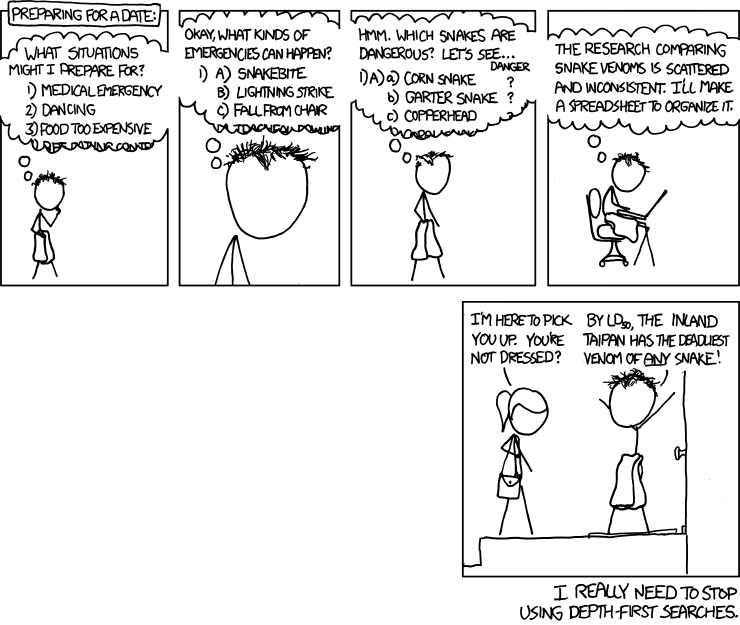
\includegraphics[width=\textwidth]{pics/dfs}
\end{center}

\noindent Despite all these issues, we will very often elect to use DFS! 
The main advantage is its very good space complexity for tree search versus 
BFS. Consider the following example with $b = 2$. The red nodes indicate the current frontier 
after expanding the blue node (6). For BFS (left), every node at this depth is being added to the 
frontier. For DFS (right), we at most have $b$ nodes on the frontier for each depth so far.
This means that DFS with Tree-Search requires far less memory than BFS, making it more practical in many settings.



\begin{center}
    \Tree [ .1 [ .2  [ .4  [ .\textcolor{red}{8} $\vdots$ ] [ .\textcolor{red}{9} $\vdots$ ] ] [ .5 [ .\textcolor{red}{10} $\vdots$ ] [ .\textcolor{red}{11} $\vdots$ ] ] ] [ .3 [ .\node[draw]{\textcolor{blue}{6}}; \textcolor{red}{12} \textcolor{red}{13} ] [ .\textcolor{red}{7} 14 15 ]  ] ]\hspace*{2cm}
    \Tree [ .1 [ .2  [ .4  [ .8 $\vdots$ ] [ .9 $\vdots$ ] ] [ .5 [ .\textcolor{black}{10} $\vdots$ ] [ .\textcolor{black}{11} $\vdots$ ] ] ] [ .3 [ .\node[draw]{\textcolor{blue}{6}}; \textcolor{red}{12} \textcolor{red}{13} ] [ .\textcolor{red}{7} 14 15 ]  ] ]
\end{center}



\subsection{Variants of DFS}

\paragraph{Depth-Limited Search}

The main issue with DFS is that it can go down paths much deeper the deepest solution $m$. 
Depth-limited search (DLS) is identical to DFS, except that we modify
the stack delete any paths beyond a fixed depth-limit is $l$.  


By
doing this we limit the space of paths it can possibly explore to
$O(b^l)$ and thus the complexity is improved. However, if $l < d$ the
algorithm is still not complete.

\begin{itemize}
\item Completeness: No.  
\item Optimality: No.
\item Time-Complexity: $O(b^l)$ 
\item Space-Complexity: $O(b^l)$ for graph-search but only $O(bl)$ for tree-search.
\end{itemize}


\noindent Note that we will implement a variant depth-limited search in the next section on game playing.

\paragraph{Iterative Deepening Search}

However, we can take this approach one step further. In iterative deepening search we repeatedly run DLS with $l = 1, \ldots$. By doing so, $l$ will eventually reach $d$ and we will find a solution. 

\begin{itemize}
\item Completeness: Yes.
\item Optimality: No. (Like BFS, optimal when all costs are 1)
\item Time-Complexity: $O(b^d)$ 
\item Space-Complexity: $O(b^d)$ 
\end{itemize}

\begin{exercise}
  Why is the time-complexity for IDS so low if we have to run it some many times?
\end{exercise}

\censor{We may have to run the algorithm at most $d$ times to find a solution. In the worst case this gives $O(b^1 + \ldots +b^d)$ time. However, in big O notation that becomes just $O(b^d)$ since the last run dominates. }

\subsection{Uniform-Cost Search}

The failure case for the optimality of BFS is when there is a deep
node that has a lower cost than a shallower node. BFS fails to be
optimal in this case, because it order paths by depth. Uniform-cost
Search (UCS) fixes this issue by ordering paths by cost instead. 

To do this we use a \textbf{priority queue} where 'pop' gives the next
path based on a priority function. Define the priority function as:
$f:\mcP \mapsto \reals$ to select the next path. For UCS, we set this
function to be $f(p)\triangleq g(p)$, i.e. the cost of the partial
path.

Here again is the algorithm applied to our example:

\begin{center}
\begin{tabular}{cccll}
  \toprule
  iter & $p$ & $s$ & frontier ($p$) & explored \\
  \midrule
  0 & - & - & \censor{[A:0]} & \censor{\{\}} \\
  1 &A & A & \censor{[A:B:2, A:D:3, A:E:5]} & \censor{\{A\}} \\
  2 &A:B & B & \censor{[A:D:3, A:E:5]} & \censor{\{A, B\}} \\
  3 &A:D & D  & \censor{[A:E:5, A:D:C:7] }& \censor{\{A, B, D\}} \\
  4 &A:E & E & \censor{[A:D:C:8]} & \censor{\{A, B, D, E\}} \\
  5 &A:D:C & C & - & - \\
  \bottomrule
\end{tabular}
\end{center}


Because UCS expands paths in cost order and costs are non-negative,
each path it expands must be at least as costly as all previous paths.
This means that if UCS finds a goal node it must be optimal. With a few 
further assumptions (see AIMA) we can also show it is complete. AIMA also 
includes a description of the time- and space-complexity that uses 
the optimal score and smallest path cost $\epsilon$. 

\begin{itemize}
\item Completeness: Yes.  
\item Optimality: Yes.
\item Time-Complexity: $O(b^{1 +\lfloor C^*/\epsilon \rfloor } )$ 
\item Space-Complexity: $O(b^{1 +\lfloor C^*/\epsilon \rfloor } )$
\end{itemize}


\section{Informed Search}

Up to this point we assumed that we have no further knowledge into the
nature of the search model. With this requirement there is no hope to
find an optimal solution without first expanding all path with cost $<
C*$ (as in UCS).  However it in practice we often have more insight
into the structure of the problem, for instance roughly how close we 
are to a goal state. When we have this information we can instead run 
informed search.

\subsection{Heuristic Functions}

A \textbf{heuristic} function provides an estimate of the cost from 
any state to a goal state.  

Consider the path finding problem. If we know that we are in
two-dimensions and the path costs correspond to distances, we can
compute the \textbf{straight-line} distance to the goal from each
state. Figure~\ref{fig:heu} shows the path finding problem with these
values overlaid. Of course in practice we cannot travel directly
from A to C or from B to C, but we will see that this extra
information can be used to help us find a solution.

% As a second example, consider again the problem of automatic
% translation. Recall that here a state consists of some English words and 
% a list of Spanish words that have been used so far. It turns out that 
% it is fast to finish off the translation if we don't have to keep track 
% of the words that we have used so far. We can quickly get a estimate 
% of the cost by allowing the model to translate words multiple times.  
% Figure~\ref{fig:heu} gives one way of completing the translation.


\begin{figure}
  \centering

  \begin{tikzpicture}
    \Graph
    \draw[dashed,red] (A)--node[yshift=0.2cm]{6} (C); 
    \draw[dashed,red] (B)--node[yshift=-0.2cm]{6} (C); 
  \end{tikzpicture}
% }
%   \subfloat[]{
  % \begin{tikzpicture}
  %   \matrix(dict)[matrix of nodes, ampersand replacement=\&]{
  %     Mary \& golpeo \& la \& bruja \& verde \\
  %     ~\\
  %     ~\\
  %     Mary \& slapped \& \node[red]{the};  \& \node[red]{green}; \& \node[red]{green};\\ };
  %   \path[draw, ->] (dict-1-1) -> (dict-4-1);
  %   \path[draw, ->] (dict-1-2) -> (dict-4-2);
  %   \path[draw, dashed, red, ->] (dict-1-3) -> (dict-4-3);
  %   \path[draw, dashed, red, ->] (dict-1-5) -> (dict-4-4);
  %   \path[draw, dashed, red,->] (dict-1-5) -> (dict-4-5);
  % \end{tikzpicture}
% }
  \caption{\label{fig:heu} An example heuristic: straight-line distance.}
\end{figure}


% \begin{itemize}
% \item You are on a road-trip and you want to minimize your cost to getting home. You see a sign that say 180 miles to New York. You think well I am driving around 60 MPH so I'll be home in about 3 hours. 
% \item For translation, you may ignore the order of the words in English. You think what if the best translation was just translating each word by itself.   
% \end{itemize}


% So far we have been assuming that the search problem is a black-box. 



Formally, a heuristic function is just any estimation of this cost from the state itself. 
% In practice though, we often know something about the problem we are interested in. Maybe we know roughly how... 


\begin{center}
\begin{tabularx}{\linewidth}{llX}
  \toprule \\
 Heuristic & $h: \mcS \mapsto \reals$ & Estimate of the cost from state $s$ to a goal state. \\\\
\bottomrule
\end{tabularx}
\end{center}



% Utilizing this value we define the \textbf{estimated cost} $f: \mcP \mapsto \reals$, of a path to the goal. 

% % Informally consider the following examples of heuristics. 



% % All of the methods we look at today are extensions on Uniform cost search, that is they will all utilize a priority queue. The main difference will be in what value they use to order the queue. 

% We call this value the  \textbf{estimated cost}, $f: \mcP \mapsto \reals$, of a path to the goal. 


\subsection{Greedy Best-First Search}

In greedy best-first search, we use the same algorithm as UCS, but instead use a priority function that substitutes in the heuristic value of the last state of the path, that is: 

\[f(p) = h(p_s) \]  

In this algorithm we always expand the node that the heuristic thinks has the smallest cost to go to a goal. In a way if UCS is conservative like BFS, this algorithm is greedy like DFS.

The benefit of this method is that with a good heuristic it can find a solution very quickly, since it doesn't waste time refining shallower paths. The downside is that we have no guarantee about the cost of the solution is. In fact the expansion order does not even take account the cost of the path that is expanded. 
   

\begin{itemize}
\item Completeness: No.  
\item Optimality: No. 
\item Time-Complexity: $O(b^m)$
\item Space-Complexity: $O(b^m)$ 
\end{itemize}

\subsection{A$^*$ Search}

The lesson from greedy best-first search is that the heuristic can be useful for directing expansion, but it should be combined with some notion of the cost of the path so far. 

This is the insight behind A$^*$ search, which is one of the most important algorithms we will discuss in this class. Like Greedy Best-First Search $A^*$ uses a priority queue but with the modified priority function.

\[f(p) \triangleq g(p) + h(p_s) \]  


Let's consider plugging this cost into our path-finding problem. 

\begin{center}
\begin{tabular}{cccll}
  \toprule
  iter & $p$ & $s$ & frontier ($p$) & explored \\
  \midrule
  0 & - & - & \censor{[A=0+6]} & \censor{\{\}} \\
  1 &A & A & \censor{[ A:D=3+4, A:B=2+6, A:E=5+4]} & \censor{\{A\}} \\
  2 &A:D & D & \censor{[A:D:C:7+0, A:B=2+6, A:E=5+4]} & \censor{\{A, D\}} \\
  3 &A:D:C & C  & -& - \\
  \bottomrule
\end{tabular}
\end{center}

\noindent Note that A$*$ not only finds the optimal solution, but it does so in 
a smaller number of iterations than the other algorithms. In fact for this problem
it uses the minimal number of expansions.

\subsection{A$*$ Properties} 

Now let us consider using A$^*$ with a heuristic $h$ satisfying the following properties.

\begin{defn}
  An \textbf{admissible} heuristic never overestimates the cost to a goal state, i.e.  \[g(p) +
  h(p_s) \leq g(\hat{p})\] where $\hat{p}\in \mcQ$ is any solution path with 
  $p$ as a partial path.
\end{defn}

\begin{defn}
  A  \textbf{consistent} heuristic obeys the property that for any state $s$, \[h(s) \leq c(s, a)
  + h(\msc{Res}(s, a))\]
 for all
  actions $a \in \msc{Act}(s, a)$.
\end{defn}

Consistency is a stronger condition and implies admissibility. However, there are cases where just admissibility is sufficient so we define both.


This leads us to the crucial theorem for informed search.

\begin{theorem}
  $A^*$ ordering  with a consistent heuristic yields an optimal search algorithm.
\end{theorem}

\noindent \textbf{Proof:}

We first prove that the A$^*$ estimated cost increase at each expansion, and then use this to show that the first expansion of any state is optimal. This implies that the first time we expand a goal state is optimal.  

\begin{enumerate}
\item The values of expanded paths are non-decreasing.

Assume we have expanded a path $p$ to a path $p'$ with action $a$, we have:

\ifthenelse{\isundefined{\StudentVersion}}{
\censor{}
\begin{eqnarray*}
f(p') &=& g(p') + h(p_s') = g(p) + c(p_s, a) + h(p'_s)  \\
&\geq & g(p) + h(p_s) =f(p),
\end{eqnarray*}
}{

\censor{}
\vspace{1cm}
}

\noindent Where we have directly used the definition of consistency for the inequality.

\item Whenever $A^*$ expands a path, the optimal path to that node has already been found. 

We will prove this by contradiction. 

Say we have expand path $p$ before the optimal path to this state $q$. This means that $p_{\mathrm{last}} =q_\mathrm{last}$ and  $g(q) < g(p)$, this implies $f(q) < f(p)$.

Since we expanded $p$ first, this also mean there is some partial path
of $q$ called $q'$ in the frontier that currently has $f(p) \leq f(q')$ (or else it
would have been expanded first).

However by Property~(1) we know that as a partial path of $q$, $f(q') \leq f(q)$. 

Together this gives a contradiction:

\ifthenelse{\isundefined{\StudentVersion}}{
\censor{}
\[ f(q) < f(p) \leq f(q') \leq f(q) \] 
}{
\vspace{1cm}
\censor{}

}



\end{enumerate}
\QED

\noindent Property~(2) implies that whenever $A^*$ expands the goal state it must be the optimal path to the goal.

\begin{itemize}
\item Completeness: Yes.  
\item Optimality: Yes. 
\item Time-Complexity: $O(b^\Delta)$ (depends on the absolute error of $h$, see AIMA3e, p.98)
\item Memory-Complexity: $O(b^\Delta)$ (graph search)
\end{itemize}


\subsection{Heuristics for Path-Finding}

Now let's return to the heuristics we discussed above. How can we check whether they satisfy the properties necessary for A$^*$ search? First consider straight-line distance. We would like to show that for any state $s$ and valid action $a$:

\[h(s) \leq c(s, a) + h(\msc{Res}(s, a))\]

\noindent and let's call the resulting state $s' = \msc{Res}(s, a)$.

We have defined our problem such that the cost of the action is the distance between $s$ and $s'$, i.e. $d(s, s')$. And we have defined our heuristic $h(s)$ as the distance to our goal $h(s) = d(s, \mathrm{C})$. So for consistency we need to show that: 



\ifthenelse{\isundefined{\StudentVersion}}{
\censor{}\[d(s, \mathrm{C}) \leq d(s, s') + d(s', \mathrm{C})\]

\noindent However this is just the triangle inequality! Since this holds for Euclidean distance, we have consistency for this problem.
}{
\vspace{1cm}
\censor{}

}

\subsection{Comparing Heuristic Functions}

While all consistent heuristics will find an optimal solution, not all
consistent heuristics are equal. As you will discover first hand in
the homework, a better heuristic will find the optimal solution much
quicker, and in fact the time and memory complexity of A$*$ depend on 
the quality of the heuristic. A better heuristic will produce a smaller
absolute error $\delta$, where delta is the difference from the completing 
path $\hat{p}^*$.

\[\delta(p, s) = g(\hat{p}^*) - (g(p) + h(p_s)) \] 

We can use this to compare different heuristics. Basically we would like 
the heuristic that produces the highest estimate while still maintaining 
consistency.

\begin{defn}
  Given two consistent heuristics $h$ and $h'$, we say $h$ \textbf{dominates} $h'$ if 
  for all $s\in\mcS$, $h(s) \geq h'(s)$. 
\end{defn}

In the simplest case, if we have two heuristics $h_1$ and $h_2$, we
can construct an admissible heuristic that is at least as good by
taking $h(s) = \max\{ h_1(s), h_2(s)\}$.

\begin{exercise}
  Show that this heuristic $h$ is still admissible.
\end{exercise}
    
In section we will further explore various.

\subsection{Generating Heuristic Functions}

A harder question though is how to generate consistent heuristics for arbitrary problems. How do we come up with heuristic for real problems? And how do we show that they satisfy consistency? 

One method for doing is known as \textbf{relaxation}. Generally the approach works like this:

\begin{itemize}
\item Write down the explicit constraints that are required for the problem. 
\item Select a subset of these constraints to ``relax''.
\item Calculate the optimal solution without these constraints and use as heuristic.   
\end{itemize}

Oftentimes when the constraints are dropped the problem becomes much more efficient to solve, and it leads to an admissible heuristic since we are making it strictly easier to reach any goal.

For path-finding we relaxed the problem by assuming we did not have to follow any of the paths directly. This allows get an underestimate of the solution. For translation, our problem assumed that each word was translated exactly once. Our heuristic is to relax this constraint and allow any remaining word translated multiple times. We can compute this heuristic cost very efficiently, and it gives us an underestimate of the optimal. 




\subsection{Relaxation Example: 8-Puzzle}

In practice, coming up with good relaxations is the key for finding efficient, optimal search algorithms. In your homework, you will construct various heuristics for difficult maze problems. To help with this, in section, we will go over examples of relaxations. In particular we will look at the various heuristics developed for the 8-Puzzle problem below: 

\begin{center}
  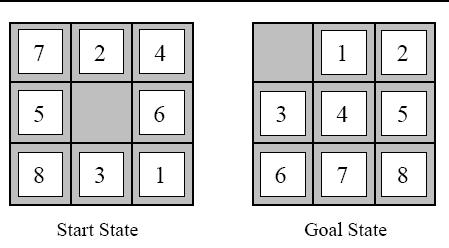
\includegraphics{pics/puzzle}
\end{center}

% If we are clever this heuristic cost can be made very efficient by precomputing values. 

% AIMA gives several more examples of effective heuristic for difficult search problems.

\end{document}
